\documentclass[11pt]{article}
\usepackage{../../latex/stat4ml_style}

\title{Chapter 7: Clustering \\ \large Part II --- Introduction to Statistical Learning}
\author{Omid Safarzadeh}
\date{}

\begin{document}
\maketitle

\begin{abstract}
\noindent
Clustering asks the hardest version of an unsupervised question: with no
labels at all, can we find the groups the data falls into? This chapter
treats the workhorse, $k$-means, not as a recipe but as \emph{coordinate
descent} on a single objective --- which is exactly why its two familiar
steps, ``assign to the nearest centre'' and ``move each centre to its
points' mean'', can never make the clustering worse, and why it always stops.
From there we place it in a family: soften the assignments and it becomes the
Gaussian mixture of Chapter~6; drop the idea of centres altogether and cluster
by density instead, and you get DBSCAN, which finds clusters that are not
blobs and calls the leftover points noise.
\end{abstract}

\tableofcontents

% ======================================================================
\section{The problem, and an objective to minimise}
% ======================================================================

We are given points $x_1,\dots,x_n$ and a number of groups $K$, and nothing
else --- no labels to predict, no right answer to check against. A
\keyterm{clustering} is an assignment of each point to one of the $K$ groups.
To make ``good grouping'' precise, $k$-means picks a \keyterm{centroid}
$\mu_k$ for each group and scores a clustering by how tightly the points sit
around their own centroid.

\begin{definition}[The $k$-means objective]
Let $c_i\in\{1,\dots,K\}$ be the cluster of point $x_i$ and $\mu_1,\dots,\mu_K$
the centroids. The \keyterm{within-cluster sum of squares} (the
\emph{inertia}) is
\[
  J(c,\mu) \;=\; \sum_{i=1}^{n} \bigl\| x_i - \mu_{c_i} \bigr\|^2 .
\]
$k$-means seeks the assignment $c$ and centroids $\mu$ that make $J$ as small
as possible.
\end{definition}

Minimising $J$ over \emph{all} assignments at once is NP-hard, so we do not try.
Instead we exploit the shape of $J$: it depends on two sets of unknowns, the
assignments $c$ and the centroids $\mu$, and if either one is held fixed the
best choice of the other is immediate. Optimising one block at a time with the
other frozen is \keyterm{coordinate descent}, and that is all Lloyd's
algorithm is.

% ======================================================================
\section{$k$-means is coordinate descent}
% ======================================================================

Two one-line facts do the work. Each says: with the other block fixed, here is
the exact minimiser.

\begin{theorem}[The assignment step is optimal]
With the centroids $\mu$ fixed, $J$ is minimised by sending each point to its
nearest centroid, $c_i = \arg\min_k \|x_i-\mu_k\|^2$.
\end{theorem}
\begin{proof}
$J=\sum_i \|x_i-\mu_{c_i}\|^2$ is a sum of non-negative terms, one per point,
and point $i$ influences only its own term through $c_i$. Minimising a sum of
independent terms means minimising each term, and the smallest
$\|x_i-\mu_k\|^2$ over $k$ is attained at the nearest centroid.
\end{proof}

\begin{theorem}[The update step is optimal]
With the assignments $c$ fixed, $J$ is minimised by setting each centroid to
the mean of the points assigned to it,
$\mu_k = \tfrac{1}{|C_k|}\sum_{i\in C_k} x_i$, where $C_k=\{i:c_i=k\}$.
\end{theorem}
\begin{proof}
With $c$ fixed, $J$ splits across clusters, $J=\sum_k \sum_{i\in C_k}\|x_i-\mu_k\|^2$,
so each $\mu_k$ can be chosen separately. The function
$g(\mu)=\sum_{i\in C_k}\|x_i-\mu\|^2$ is convex; setting its gradient to zero,
\[
  \nabla g(\mu) = -2\sum_{i\in C_k}(x_i-\mu) = 0
  \quad\Longrightarrow\quad
  \mu = \frac{1}{|C_k|}\sum_{i\in C_k} x_i .
\]
So the minimiser is exactly the cluster mean --- which is where the name
comes from.
\end{proof}

Alternating the two is \keyterm{Lloyd's algorithm}:

\begin{lstlisting}[language=Python]
def kmeans(data, centroids, n_iter=100):
    for _ in range(n_iter):
        # E-like step: assign each point to the nearest centroid
        labels = [min(range(len(centroids)),
                      key=lambda k: sq_dist(x, centroids[k])) for x in data]
        # M-like step: move each centroid to the mean of its points
        new = []
        for k in range(len(centroids)):
            members = [data[i] for i in range(len(data)) if labels[i] == k]
            new.append(mean(members) if members else centroids[k])
        if new == centroids:            # nothing moved -> converged
            break
        centroids = new
    return labels, centroids
\end{lstlisting}

\noindent The figure runs exactly this from a deliberately poor
initialisation: the centroids start bunched together, and within a handful of
passes they settle on the three blobs. The right-hand panel is the point of
the whole section --- the objective $J$ falls at every step and then flattens.

\begin{figure}[h]
  \centering
  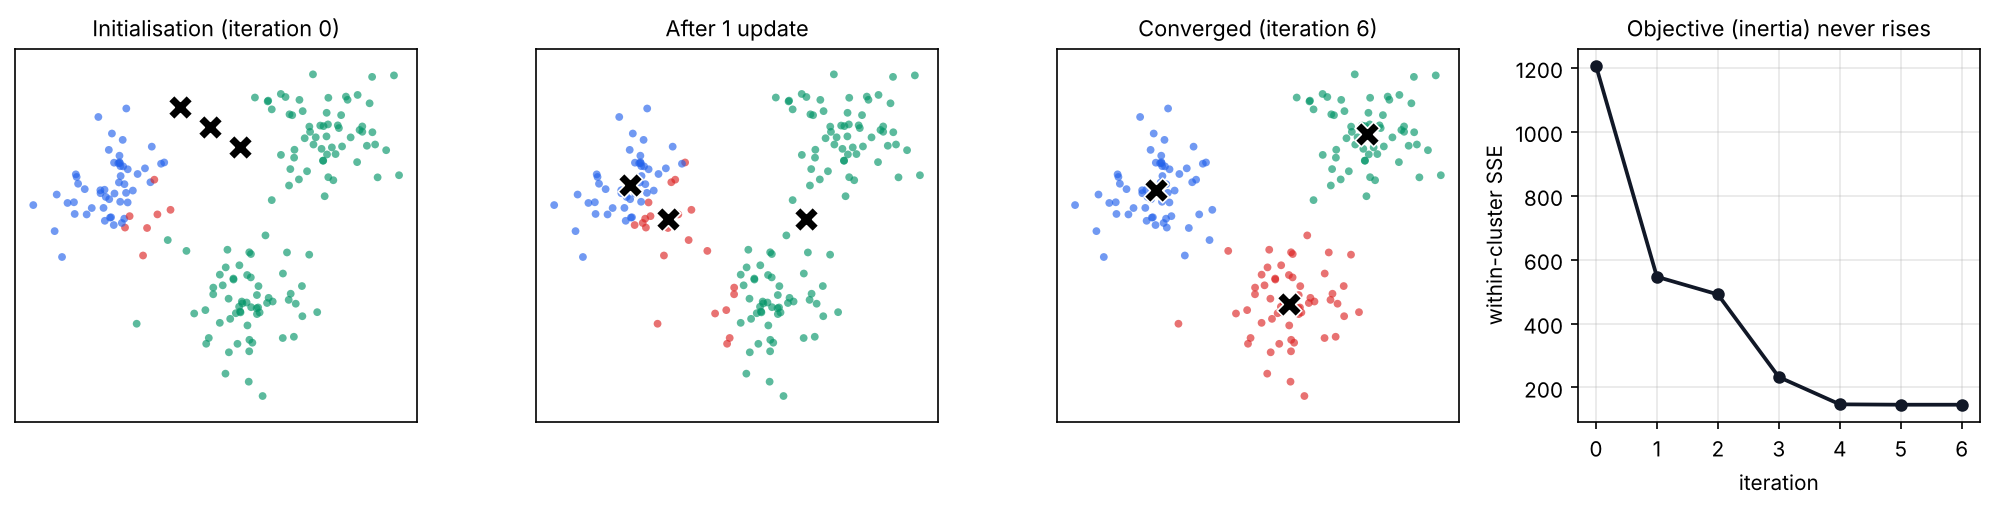
\includegraphics[width=\linewidth]{figures/kmeans_panel.png}
\end{figure}

\begin{theorem}[Lloyd's algorithm converges]
The sequence of objective values produced by Lloyd's algorithm is
non-increasing, and the algorithm terminates in finitely many iterations.
\end{theorem}
\begin{proof}
Each iteration is two minimisations of the \emph{same} $J$: the assignment
step cannot increase $J$ (Theorem~2.1) and the update step cannot increase it
either (Theorem~2.2), so $J$ is non-increasing. There are only finitely many
possible assignments $c$ (at most $K^n$), and given $c$ the optimal centroids
are determined, so each distinct assignment has one objective value. A
non-increasing sequence that can never revisit a higher value and draws from a
finite set must stabilise; once $J$ stops strictly decreasing the assignments
stop changing, and the algorithm halts.
\end{proof}

A caution the proof makes honest: coordinate descent finds a \emph{local}
minimum, not the global one. The value it lands on depends on where the
centroids start, which is why practitioners run $k$-means several times from
different seeds and keep the lowest $J$ --- and why \keyterm{$k$-means\texttt{++}},
which spreads the initial centroids out by sampling each new one with
probability proportional to its squared distance from the nearest chosen
centre, is the standard way to seed it.

% ======================================================================
\section{Softer and denser: GMMs and DBSCAN}
% ======================================================================

$k$-means makes two strong commitments: every point belongs fully to one
cluster, and a cluster is whatever is closest to a centre --- so clusters come
out as round, equal-sized blobs. Relaxing each commitment gives a different
method.

\paragraph{Soft assignments: the Gaussian mixture.}
Let a point belong \emph{partly} to several clusters and you are back at the
\keyterm{Gaussian mixture model} of Chapter~6. There the responsibility
$r_{ik}=\pi_k f_k(x_i)/\sum_j \pi_j f_j(x_i)$ replaces the hard label, and EM's
E-step and M-step are the soft echoes of assign-and-update. In fact $k$-means
is the limit of EM on a Gaussian mixture when every component is forced to the
same spherical covariance and that covariance shrinks to zero: the soft
responsibilities harden to a single winning cluster, and the two algorithms
coincide. The gain from staying soft is that a GMM can fit elliptical,
unequal, overlapping clusters that $k$-means cannot.

\paragraph{No centres at all: density clustering.}
\keyterm{DBSCAN} drops centroids entirely and clusters by \emph{density}. Fix a
radius $\varepsilon$ and a count $m$. A point is a \keyterm{core point} if at
least $m$ points lie within distance $\varepsilon$ of it; core points that are
within $\varepsilon$ of each other are chained into the same cluster, border
points are attached to a nearby core, and anything left over is labelled
\keyterm{noise}.

\begin{definition}[Core point]
Point $x$ is a core point at scale $(\varepsilon, m)$ if
$\bigl|\{\,j : \|x_j - x\| \le \varepsilon\,\}\bigr| \ge m$,
counting $x$ itself.
\end{definition}

\noindent Because clusters grow by following density rather than distance to a
centre, DBSCAN finds clusters of any shape --- two interleaving crescents, a
ring around a blob --- that no centroid method can separate, and it needs no
$K$ in advance: the number of clusters falls out of the data. Its price is
sensitivity to $\varepsilon$, and trouble when different clusters have very
different densities.

\begin{example}[Which method for which data]
Round, well-separated, roughly equal groups and you know $K$: $k$-means, fast
and enough. Overlapping or elliptical groups where you want a probability of
membership: a Gaussian mixture. Oddly shaped clusters, unknown $K$, or real
noise to reject: DBSCAN.
\end{example}

\begin{summarybox}
Clustering groups unlabelled points. $k$-means minimises the within-cluster
sum of squares $J(c,\mu)=\sum_i\|x_i-\mu_{c_i}\|^2$ by coordinate descent:
assigning each point to its nearest centroid and moving each centroid to its
points' mean are the exact minimisers of $J$ over one block with the other
fixed, so $J$ is non-increasing and Lloyd's algorithm converges --- to a
\emph{local} optimum, hence multiple restarts and $k$-means\texttt{++}
seeding. Softening the hard assignment gives the Gaussian mixture of
Chapter~6, of which $k$-means is the zero-variance limit; dropping centres for
density gives DBSCAN, which clusters arbitrary shapes, infers the number of
clusters, and labels outliers as noise.
\end{summarybox}

\end{document}
